

\section{CTI Benchmark Results}
\label{sec:cti-results}

\subsection{Task-Level Results and Paired Comparisons}
\label{sec:main-results}

\begin{table}[t]
\centering
\scriptsize
\caption{Per-task paired bootstrap 95\% confidence intervals for MinervaRL minus GRPO, in percentage points. Positive intervals indicate tasks where MinervaRL is higher than GRPO under the paired bootstrap interval.}
\label{tab:grpo-pairwise-ci}
\setlength{\tabcolsep}{3pt}
\renewcommand{\arraystretch}{0.92}
\resizebox{0.7\textwidth}{!}{%
\begin{tabular}{lrrrr}
\toprule
Task & Llama-3.1-8B & Llama-3.2-3B & Qwen3-8B & Qwen3-4B \\
\midrule
CKT & +2.0 [0.6, 3.5] & -0.2 [-1.6, 1.1] & +8.0 [6.5, 9.5] & -4.2 [-5.8, -2.6] \\
CyberMetric & -1.1 [-2.5, 0.3] & +0.3 [-1.1, 1.5] & +15.5 [13.5, 17.5] & -5.7 [-7.4, -4.0] \\
SOCEval & +1.7 [-0.4, 3.8] & -3.7 [-5.8, -1.4] & -1.4 [-2.7, -0.1] & +0.2 [-1.6, 2.1] \\
RCM & +2.4 [1.1, 3.8] & +8.3 [6.8, 9.8] & +4.3 [2.9, 5.8] & -0.9 [-2.1, 0.2] \\
VSP & +5.0 [4.3, 5.7] & +20.6 [18.9, 22.4] & +10.6 [9.7, 11.7] & -8.1 [-9.0, -7.3] \\
ATE & +16.4 [12.6, 20.4] & +16.6 [13.2, 20.2] & +8.4 [5.8, 11.4] & +5.2 [2.8, 7.6] \\
RMS & +11.2 [7.8, 14.4] & +13.9 [11.1, 16.9] & +12.0 [9.1, 14.8] & +1.3 [-0.7, 3.2] \\
ElasticRule & +8.3 [3.9, 12.7] & +14.8 [11.6, 18.3] & +3.9 [-0.2, 7.9] & +7.2 [3.7, 10.9] \\
APTNER & +1.4 [0.5, 2.4] & -10.8 [-12.3, -9.3] & -0.3 [-1.5, 1.0] & -4.4 [-5.9, -2.9] \\
LANCE & -1.5 [-5.7, 2.2] & +11.7 [2.7, 19.3] & +8.8 [0.8, 19.9] & -1.5 [-10.5, 9.3] \\
AnnoCTR & +0.7 [-1.6, 2.9] & -0.7 [-2.4, 1.1] & +5.2 [3.2, 8.1] & +10.7 [4.4, 12.9] \\
AZERG & +4.1 [2.3, 7.7] & +4.0 [1.5, 7.0] & +2.0 [0.1, 5.6] & +5.1 [0.3, 7.8] \\
\bottomrule
\end{tabular}%
}
\end{table}

\begin{table}[t]
\centering
\scriptsize
\caption{Pairwise task-count summary for MinervaRL versus each baseline across 48 backbone-task comparisons. CI Pos. and CI Neg. are counts of comparisons whose paired 95\% confidence interval is entirely above or below zero.}
\label{tab:pairwise-ci-summary}
\setlength{\tabcolsep}{4pt}
\renewcommand{\arraystretch}{0.95}
\begin{tabular}{lccccc}
\toprule
Baseline & Point wins & Point losses & CI Pos. & CI Neg. & CI Overlap \\
\midrule
Base & 42/48 & 6/48 & 35/48 & 2/48 & 11/48 \\
STaR & 38/48 & 10/48 & 35/48 & 6/48 & 7/48 \\
DART & 38/48 & 10/48 & 34/48 & 3/48 & 11/48 \\
GRPO & 34/48 & 14/48 & 28/48 & 7/48 & 13/48 \\
LUFFY & 32/48 & 16/48 & 20/48 & 6/48 & 22/48 \\
\bottomrule
\end{tabular}
\end{table}

\paragraph{Aggregate task scores.}
\Cref{tab:main-results} reports absolute scores across the 12 CTI evaluation tasks and four open-weight backbone families. Standard GRPO improves the average score over each matched base model, raising Llama-3.1-8B from 48.6 to 56.0, Llama-3.2-3B from 33.1 to 42.1, Qwen3-8B from 37.6 to 47.0, and Qwen3-4B from 27.6 to 47.6. These gains are largest on structured verifier-aligned tasks such as CWE mapping, CVSS prediction, ATT\&CK technique identification, mitigation recommendation, and rule-to-technique mapping. MinervaRL further raises the average to 60.2, 48.3, 53.4, and 48.0 for the four backbones, respectively, obtaining the highest average score within each backbone group.

\paragraph{Comparison with controlled baselines.}
Compared with STaR-CTI and DART-CTI, MinervaRL has a higher average score for all four backbone groups. LUFFY-CTI is the closest controlled baseline: MinervaRL is higher by +3.2 points on Llama-3.1-8B, +2.9 on Llama-3.2-3B, +0.2 on Qwen3-8B, and +4.0 on Qwen3-4B. On Llama-3.1-8B, MinervaRL also exceeds the two external security-SFT reference models, reaching 60.2 average compared with 50.2 for Llama-Primus-Merged and 51.9 for Foundation-Sec-8B-Instruct.

\paragraph{Per-task paired uncertainty versus GRPO.}
To complement the aggregate scores, \Cref{tab:grpo-pairwise-ci} reports per-task paired bootstrap 95\% confidence intervals over evaluation examples for MinervaRL minus GRPO. Across the 48 backbone-task comparisons, MinervaRL has positive point deltas on 34/48 comparisons; the paired interval is entirely above zero on 28/48, entirely below zero on 7/48, and overlaps zero on 13/48. The strongest CI-separated gains are concentrated on structured verifier-aligned tasks including RCM, VSP, ATE, RMS, and ElasticRule. The Qwen3-4B comparison is the least separated: its average gain over GRPO is small, and several task-level intervals are negative or overlap zero.

\paragraph{Pairwise summary across baselines.}
\Cref{tab:pairwise-ci-summary} summarizes paired interval signs for MinervaRL against each baseline across all 48 backbone-task comparisons. MinervaRL is higher than the base models on 42/48 point comparisons, with 35/48 CI-positive intervals. It also has broad CI-positive majorities against STaR-CTI and DART-CTI, with 35/48 and 34/48 CI-positive intervals, respectively. Against LUFFY-CTI, the closest controlled baseline, MinervaRL has positive point deltas on 32/48 comparisons; the paired 95\% interval is entirely above zero on 20/48, entirely below zero on 6/48, and overlaps zero on 22/48.

\subsection{Task-Family Summary}
\label{sec:task-family-summary}

\begin{table}[t]
\centering
\scriptsize
\caption{Task-family count summary for MinervaRL versus each baseline. Counts are over backbone-task comparisons within each family. Point W/L reports MinervaRL point wins/losses; CI +/-/0 reports CI-positive, CI-negative, and CI-overlap counts.}
\label{tab:task-family-count-summary}
\setlength{\tabcolsep}{3pt}
\renewcommand{\arraystretch}{0.92}
\resizebox{0.95\textwidth}{!}{%
\begin{tabular}{@{}l|cc|cc|cc|cc@{}}
\toprule
& \multicolumn{2}{c|}{QA / selection (n=12)}
& \multicolumn{2}{c|}{Taxonomy mapping (n=16)}
& \multicolumn{2}{c|}{Vulnerability scoring (n=4)}
& \multicolumn{2}{c}{Information extraction (n=16)} \\
\cmidrule(lr){2-3}
\cmidrule(lr){4-5}
\cmidrule(lr){6-7}
\cmidrule(lr){8-9}
Baseline
& Point W/L & CI +/-/0
& Point W/L & CI +/-/0
& Point W/L & CI +/-/0
& Point W/L & CI +/-/0 \\
\midrule
Base  & 9/3  & 7/0/5 & 15/1 & 15/1/0 & 4/0 & 4/0/0 & 14/2 & 9/1/6 \\
STaR  & 9/3  & 9/2/1 & 15/1 & 15/1/0 & 3/1 & 3/0/1 & 11/5 & 8/3/5 \\
DART  & 10/2 & 9/1/2 & 15/1 & 15/0/1 & 4/0 & 4/0/0 & 9/7  & 6/2/8 \\
GRPO  & 6/6  & 3/4/5 & 15/1 & 13/0/3 & 3/1 & 3/1/0 & 10/6 & 9/2/5 \\
LUFFY & 8/4  & 4/0/8 & 10/6 & 8/3/5  & 4/0 & 4/0/0 & 10/6 & 4/3/9 \\
\bottomrule
\end{tabular}%
}
\end{table}

\begin{table}[t]
\centering
\scriptsize
\caption{Llama-3.1-8B component ablations on validation splits and the 12 CTI evaluation tasks. Validation columns report Minerva-Dev and AthenaBench-Mini scores. Evaluation columns report the 12-task macro average and paired bootstrap interval sign counts across the 12 tasks. Underlined values indicate the best score in each validation or 12-task average column.}
\label{tab:eval12-ablation-summary}
\setlength{\tabcolsep}{3pt}
\renewcommand{\arraystretch}{0.95}
\resizebox{0.75\textwidth}{!}{%
\begin{tabular}{@{}l|ccc|cccc@{}}
\toprule
Ablation
& \multicolumn{3}{c|}{Validation}
& \multicolumn{4}{c}{12 CTI evaluation tasks} \\
\cmidrule(lr){2-4}\cmidrule(lr){5-8}
& \shortstack{Minerva-\\Dev}
& \shortstack{AthenaBench-\\Mini}
& Avg.
& Avg.
& CI Pos.
& CI Neg.
& CI Overlap \\
\midrule
GRPO & 50.3 & 57.4 & 53.8 & 56.0 & 8 & 0 & 4 \\
GRPO 12 rollouts & 50.9 & 52.7 & 51.8 & 53.9 & 7 & 1 & 4 \\
Answer-only SFT & 58.6 & 38.7 & 48.7 & 52.6 & 7 & 3 & 2 \\
In-loop answer SFT & 58.3 & 57.8 & 58.0 & 57.8 & 6 & 4 & 2 \\
No EMA teacher & 63.1 & 62.2 & 62.6 & 57.2 & 8 & 0 & 4 \\
No TextCNN filter & \underline{64.2} & 59.0 & 61.6 & 57.7 & 7 & 1 & 4 \\
No filtering & 63.0 & 61.4 & 62.2 & 57.8 & 7 & 0 & 5 \\
Full MinervaRL & 63.2 & \underline{63.3} & \underline{63.3} & \underline{60.2} & -- & -- & -- \\
\bottomrule
\end{tabular}%
}
\end{table}

To summarize the heterogeneous CTI evaluation tasks by output and scoring type, \Cref{tab:task-family-count-summary} groups the pairwise comparisons from \Cref{tab:pairwise-ci-summary} into four task families: QA/selection (CKT, CyberMetric, SOCEval), taxonomy mapping (RCM, ATE, RMS, ElasticRule), vulnerability scoring (VSP), and information extraction (APTNER, LANCE, AnnoCTR, AZERG). The denominators count task-by-backbone comparisons. By point wins, MinervaRL has a majority in every family-baseline block except QA/selection versus GRPO, where the comparison is tied at 6 wins and 6 losses. The same exception appears under CI-sign counts: CI-positive counts exceed CI-negative counts in every family-baseline block except QA/selection versus GRPO, where the signs are 3 positive, 4 negative, and 5 overlapping. The strongest interval-separated gains remain on taxonomy mapping and vulnerability scoring, while QA/selection and extraction tasks are more mixed.

\subsection{Component Ablations}
\label{sec:eval12-ablations}

We report component ablations for Llama-3.1-8B only. We evaluate the resulting checkpoints on the two checkpoint-selection sets, Minerva-Dev and AthenaBench-Mini, and on the 12 CTI evaluation tasks from \Cref{tab:main-results}. \Cref{tab:eval12-ablation-summary} reports validation scores, 12-task averages, and paired bootstrap sign counts for Full MinervaRL minus each control across the 12 task metrics. \Cref{tab:app-eval12-ablation-scores} reports the corresponding per-task scores.

The full method has the highest 12-task average among the component controls. In \Cref{tab:eval12-ablation-summary}, GRPO is the no-ACR control, GRPO 12 rollouts controls for additional rollout sampling, and in-loop answer SFT matches the auxiliary distillation schedule while replacing ACR traces with direct final-answer targets. GRPO is 4.2 points lower, indicating that the gain is not explained by verifier RL alone. GRPO with 12 rollouts does not close the gap despite additional rollout compute. Full MinervaRL also has a higher average than in-loop answer SFT (60.2 vs. 57.8). For Full MinervaRL minus this control, 6 paired task-level intervals are positive, 4 are negative, and 2 overlap zero. Thus, direct answer-only distillation does not recover the full method on average, but the advantage of ACR distillation is not uniform across tasks. Removing the EMA teacher or filtering components yields smaller drops in the 12-task average.

\begin{figure}[t]
  \centering
  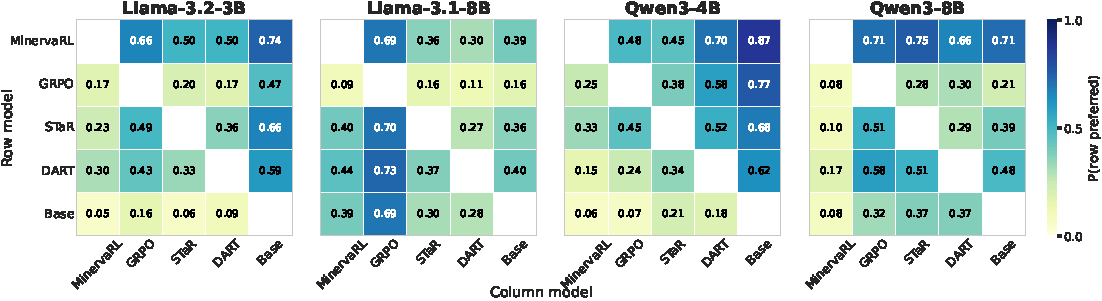
\includegraphics[width=.9\linewidth]{figures/pairwise_preference_including_ties_1x4.pdf}
  \caption{GPT-5.2 pairwise response-quality preferences for backbone-specific model groups. Each cell reports the probability that the row model is preferred over the column model, with ties retained in the denominator.}
  \label{fig:cti-judge-preference}
\end{figure}

% \subsection{In-Training vs. Not-in-Training Tasks}
% \label{sec:intrain-vs-heldout}

% \begin{table}[t]
% \centering
% \begin{minipage}{0.70\textwidth}
% \centering
% \scriptsize
% \caption{Seen vs. not-seen averages.}
% \label{tab:seen-vs-heldout}
% \setlength{\tabcolsep}{2pt}
% \renewcommand{\arraystretch}{0.88}
% \resizebox{\linewidth}{!}{%
% \begin{tabular}{l cc cc cc cc}
% \toprule
% & \multicolumn{2}{c}{Llama-3.1-8B} & \multicolumn{2}{c}{Llama-3.2-3B} & \multicolumn{2}{c}{Qwen3-8B} & \multicolumn{2}{c}{Qwen3-4B} \\
% \cmidrule(lr){2-3}\cmidrule(lr){4-5}\cmidrule(lr){6-7}\cmidrule(lr){8-9}
% Model & Seen & Not-seen & Seen & Not-seen & Seen & Not-seen & Seen & Not-seen \\
% \midrule
% Base      & 37.1 & 54.4 & 4.9  & 47.2 & 35.4 & 38.7 & 33.2 & 24.8 \\
% GRPO      & 53.0 & 57.5 & 31.5 & 47.4 & 40.3 & 50.3 & 43.2 & 49.8 \\
% MinervaRL & 61.7 & 59.5 & 46.4 & 49.3 & 49.1 & 55.5 & 42.6 & 50.7 \\
% \bottomrule
% \end{tabular}%
% }
% \end{minipage}
% \end{table}

% We split the 12 CTI evaluation tasks in \Cref{tab:main-results} into tasks that are directly seen during Minerva-CTI training (\textbf{Seen}: RCM, VSP, ATE, RMS) and tasks that are not directly optimized as training objectives (\textbf{Not-in-training}: CKT, CyberMetric, SOCEval, ElasticRule, APTNER, LANCE, AnnoCTR, AZERG). For each model variant we report the mean score over tasks in the group.



% As expected, GRPO and MinervaRL deliver the largest gains on the \emph{seen} tasks (which align closely with the verifiable training objectives), but we also observe consistent improvements on the \emph{not-in-training} tasks, indicating that training on verifiable CTI tasks transfers to related CTI reasoning and extraction capabilities.





\subsection{Response-Quality Preference Evaluation}
\label{sec:qualitative}

Verifier-based scores measure structured CTI correctness, but analyst-facing usefulness also depends on readability, evidence use, and CTI concept precision. We therefore run a blind GPT-5.2 response-quality evaluation within each backbone family, comparing the base model, GRPO, MinervaRL, STaR-CTI, and DART-CTI. Responses are scored with a three-criterion rubric covering writing quality, prompt-evidence use, and CTI concept use; pairwise preferences are derived from total scores, with ties retained. Full prompts, rubrics, and validation details are in \Cref{app:response-quality-eval}.




\paragraph{Preference results.}
\Cref{fig:cti-judge-preference} shows that MinervaRL is preferred over GRPO for all four backbones and is top-ranked for Llama-3.2-3B, Qwen3-4B, and Qwen3-8B. On Llama-3.1-8B, STaR-CTI and DART-CTI receive higher preference rates, suggesting that fixed-trace SFT and rejection-finetuning baselines can produce stronger prose for a strong instruction-tuned backbone. MinervaRL nevertheless remains preferred over the base and GRPO variants and achieves the highest average task score in \Cref{tab:main-results}, indicating that its verifier-score gains generally coincide with improved judged response quality relative to standard GRPO.

















\paragraph{Judge validation.}
We validate GPT-5.2 on a 100-example subset over the five Llama-3.1-8B-family variants, using two human annotators and Claude Sonnet 4.6. GPT-5.2 agrees substantially with the human annotator average (QWK 0.6313, Spearman 0.7722), close to human--human agreement (QWK 0.6514, Spearman 0.6461), and also agrees strongly with Claude Sonnet 4.6 (QWK 0.7634, Spearman 0.8266). Full validation results are in \Cref{app:response-quality-eval}.

\begin{table}[t]
\centering
\begin{minipage}{0.80\textwidth}
\centering
\scriptsize
\caption{Average performance on training-aligned and not-in-training evaluation tasks.}
\label{tab:seen-vs-heldout}
\setlength{\tabcolsep}{2pt}
\renewcommand{\arraystretch}{0.88}
\resizebox{\linewidth}{!}{%
\begin{tabular}{l cc cc cc cc}
\toprule
& \multicolumn{2}{c}{Llama-3.1-8B} & \multicolumn{2}{c}{Llama-3.2-3B} & \multicolumn{2}{c}{Qwen3-8B} & \multicolumn{2}{c}{Qwen3-4B} \\
\cmidrule(lr){2-3}\cmidrule(lr){4-5}\cmidrule(lr){6-7}\cmidrule(lr){8-9}
Model & Aligned & Not-in-train & Aligned & Not-in-train & Aligned & Not-in-train & Aligned & Not-in-train \\
\midrule
Base      & 37.1 & 54.4 & 4.9  & 47.2 & 35.4 & 38.7 & 33.2 & 24.8 \\
GRPO      & 53.0 & 57.5 & 31.5 & 47.4 & 40.3 & 50.3 & 43.2 & 49.8 \\
MinervaRL & 61.7 & 59.5 & 46.4 & 49.3 & 49.1 & 55.5 & 42.6 & 50.7 \\
\bottomrule
\end{tabular}%
}
\end{minipage}
\end{table}

\begin{table}[t]
\centering
\scriptsize
\caption{Task-count summary for training-aligned and not-in-training tasks among the 12 CTI evaluation tasks. Counts are over backbone-task comparisons. Aligned tasks are RCM, VSP, ATE, and RMS; not-in-training tasks are the remaining eight tasks. CI Pos./Neg./Overlap indicate whether the paired bootstrap 95\% confidence interval for MinervaRL minus the comparison model is entirely above zero, below zero, or overlaps zero.}
\label{tab:seen-vs-heldout-counts}
\setlength{\tabcolsep}{2.3pt}
\renewcommand{\arraystretch}{0.92}
\resizebox{0.8\textwidth}{!}{%
\begin{tabular}{lccccc@{\hspace{0.8em}}ccccc}
\toprule
& \multicolumn{5}{c}{Training-aligned}
& \multicolumn{5}{c}{Not-in-training} \\
\cmidrule(lr){2-6}\cmidrule(lr){7-11}
Comparison
& \shortstack{Point\\wins}
& \shortstack{Point\\losses}
& \shortstack{CI\\Pos.}
& \shortstack{CI\\Neg.}
& \shortstack{CI\\Overlap}
& \shortstack{Point\\wins}
& \shortstack{Point\\losses}
& \shortstack{CI\\Pos.}
& \shortstack{CI\\Neg.}
& \shortstack{CI\\Overlap} \\
\midrule
MinervaRL vs Base & 15/16 & 1/16 & 15/16 & 1/16 & 0/16 & 27/32 & 5/32 & 21/32 & 1/32 & 10/32 \\
MinervaRL vs GRPO & 14/16 & 2/16 & 13/16 & 1/16 & 2/16 & 20/32 & 12/32 & 15/32 & 6/32 & 11/32 \\
\bottomrule
\end{tabular}%
}
\end{table}

\subsection{Training-Aligned vs. Not-in-Training Tasks}
\label{sec:intrain-vs-heldout}

We split the 12 CTI evaluation tasks into tasks that directly match Minerva-CTI training objectives and tasks that are not directly optimized during training. The training-aligned group contains RCM, VSP, ATE, and RMS, corresponding to CVE-to-CWE mapping, CVSS vector prediction, ATT\&CK technique prediction, and mitigation recommendation. The not-in-training group contains CKT, CyberMetric, SOCEval, ElasticRule, APTNER, LANCE, AnnoCTR, and AZERG. \Cref{tab:seen-vs-heldout} reports the mean score for each group.

MinervaRL delivers the largest gains on training-aligned tasks, improving over the base model by +24.6, +41.5, +13.7, and +9.4 points on Llama-3.1-8B, Llama-3.2-3B, Qwen3-8B, and Qwen3-4B, respectively. It also improves over GRPO on three of the four backbones in this group. On not-in-training tasks, MinervaRL improves over GRPO for every backbone in the group average, with gains of +2.0, +1.9, +5.2, and +0.9 points. The task-count summary in \Cref{tab:seen-vs-heldout-counts} shows the same pattern at the task level: gains over the base model remain broad even outside the training objectives, while gains over GRPO are positive on a majority of not-in-training comparisons but more mixed than on training-aligned tasks. Overall, the gains are largest on verifier-aligned structured tasks; outside the training objectives, improvements are broader relative to base models and more mixed relative to GRPO.
